\chapter{Eredmények}
\pagestyle{headings}


\section{Grafit-modell}

Mint korábban említettem már, a pásztázó elektrokémiai mikroszkópiában általában egy céltárgy felszínét vizsgáljuk vagy az azon lejátszódó folyamatról szeretnénk információhoz jutni. Először egy jól ismert rendszert vizsgáltam meg, az előzőekben részletesebben jellemzett epoxi gyantába fogott grafit elektródpárt. A céltárgyat 2000 mV-al polarizáltam, katódosan és anódosan egymáshoz képest. A feltérképezett katód környezetében hidrogénion redukciójára vagyis lokális pH növekedésre, az anódos oldalon pedig oxigén gáz fejlődésre számíthatunk, a következő egyenletek szerint:

K(-): 2H$^+$ + 2e$^-$ \longrightarrow H$_2$ (redukció)

A(+):  2OH$^-$ \longrightarrow 0,5 O$_2$ + H$_2$O + 2e$^-$ (oxidáció)

A mikroméretű referenciaelektróddal készített pásztázások horizontális potenciáltérképeit a x ábrán, a vertikálisat pedig az x ábrán láthatjuk. Az elvárásnak megfelelő eredményeket kaptam, hiszen mind a vertikális mind pedig a horizontális képeken, -5 mV eltéréssel, azonos potenciáltartományba esnek a mérések eredményei. Továbbá jól látható, hogy az elektródpár tagjai a polarizáció hatására katódként (~ -295 mV körüli átlagérték) és anódként (~ -265 mV körüli átlagérték) viselkedtek, ahogy azt elvártuk. Így az eredményekből látható, hogy a tanulmányozott rendszer ténylegesen állandó, jól jellemezhető és a módszer, amit használtam alkalmazható a potenciáltérképezésre. 

\section{Vas-cink galvánpár korrózió vizsgálata}

Az előző alfejezetben bemutatott grafit céltárgy után egy vas-cink galvánpárból készült céltárgyat tanulmányoztam, melyet a Módszerek fejezetben jellemeztem részletesebben. Ez egy sokszor vizsgált és előforduló rendszer, mivel a vas ötvözeteit, illetve magát a vasat is, számos esetben vonjuk be a jobb korrózióállóság miatt cinkréteggel. Ezt a technikát a hétköznapi életben horganyzásnak hívjuk, ezzel a módszerrel jelentős mértékben csökkenthető a védett fém korróziója. Ez annak tulajdonítható, hogy a cink tölti be az Irodalom fejezetben említett áldozati anód szerepét a galvanikus kapcsolat során, mivel az egyik legaktívabb fémek közé sorolható. Tehát a cink oxidálódik a védett fém, vagyis a vas helyett. Ezzel egyidőben a vason redukció zajlik, viszont vaskioldódás nélkül. Ennek a folyamatnak is a lényege a hidrogénion redukció, így ahogy az előző alfejezetben jellemzett grafit katód esetén is, lokális pH növekedésre számíthatunk jelen esetben is. A cink anódon a következő reakciók játszódnak le:

2 Zn \longrightarrow 2 Zn$^{2+}$ + 4e$^-$ 

Zn$^{2+}$ + nH$_2$O \longrightarrow Zn(OH)$_{n2-n}$ + nH$^+$


A vas katódon pedig a következő reakciók mennek végbe:


2H$^+$ + 2e$^-$ \longrightarrow H$_2$

O$_2$ + 4H$_2$O + 4e$^-$ \longrightarrow 2H$_2$O + 4OH$^-$

A vizsgálatok potenciáltérképei az x ábrán láthatóak. Ebben az esetben külön pásztáztam, a katód és anód felületét a grafittal ellentétben. A felület homogén, vagyis a vas egész felülete katódként viselkedett a cellában a mérés alatt, ezzel alátámasztva, hogy a cinkelektród működött csak anódként. Ezt bizonyítja az eltérő mért potenciálértékek is, vagyis anódra jellemzően nagyobb, a cinknél -230 mV, körüli érték, és a vas esetében kisebb, -275 mV körüli érték, hasonlóan a grafit modell elvéhez. Illetve leolvasható, hogy a potenciáltartomány értékei a 3-3 pásztázásnak körülbelül azonos minimum és maximum értéket követnek itt is. A vas vertikális potenciálképénél (5.2 ábra A) látható egy szélesebb tartomány, mint a horizontális képeknél. Ez valószínűleg annak tulajdonítható, hogy a grafittól eltérően, ez a korróziós folyamat időben változó. A vertikális pásztázása és a horizontálisak között több idő telhetett el, ami során a reakció előre haladt már, így kaptam az eltérő értékeket a tartományra. Ha szétkapcsolnánk a cellát, a vas felületén lokális anód és katód alakulna ki, vagyis elvesztené a cink anódos védelmét. Láthatóvá válnának a felületen sárgás-barnás elszíneződések, vagyis a rozsdásodás folyamata beindulna. Ezen részek anódként viselkednek, nem tudnánk itt katódos aktivitást kimutatni. 


%\includegraphics[trim = 10mm 40mm 0mm 40mm, clip, width=0.4\textwidth, angle=-90]{img/mg_metal/liquid_uncoupled.eps} \includegraphics[trim = 10mm 40mm 0mm 40mm, clip, width=0.4\textwidth, angle=-90]{img/mg_metal/solid_uncoupled.eps}

\begin{figure}
\centering
\includegraphics[width=0.3\textwidth, angle=-90]{img/mérések/Fe_h_100.eps}\includegraphics[width=0.3\textwidth, angle=-90]{img/mérések/Fe_h_500.eps}

\includegraphics[width=0.3\textwidth, angle=-90]{img/mérések/Zn_h_100.eps}\includegraphics[width=0.3\textwidth, angle=-90]{img/mérések/Zn_h_500.eps}

\includegraphics[width=0.3\textwidth, angle=-90]{img/mérések/grafit_h_100.eps}
\includegraphics[width=0.3\textwidth, angle=-90]{img/mérések/grafit_h_300.eps}

\caption{Az említett céltárgyakról készült horizontális potenciáltérképek:
A és B a vas katód 100 um és 500 um magasságban, C és D a cink anód 100 um és 500 um magasságban és E és F a grafit katódja és anódja 100 um és 300 um magasságban mérve}
\label{fig:horizontális}
\end{figure}


\begin{figure}
\centering
\includegraphics[width=0.3\textwidth, angle=-90]{img/mérések/Fe_v.eps}
\includegraphics[width=0.3\textwidth, angle=-90]{img/mérések/Zn_v.eps}
\includegraphics[width=0.3\textwidth, angle=-90]{img/mérések/grafit_v.eps}


\caption{Az említett cáltárgyakról készült vertikális potenciáltértképek:
A a vas katód, B a cink anód és C a grafit katódja és anódja}
\label{fig:vertikális}
\end{figure}
